\chapter{Bases de numération}
\introduction{Partons sur de bonnes bases.}


On note $\N$ l'ensemble des \textit{entiers naturels} : $\N=\lbrace 0;1;2;\ldots\rbrace$.\\

Nous avons l'habitude d'utiliser la base 10 pour représenter les entiers naturels, c'est-à-dire qu'on utilise 10 symboles, appelés \textit{chiffres}
pour les écrire : 0, 1, 2, \ldots, 9.
Or il n'en a pas toujours été ainsi :
\begin{itemize}
    \item 	au \textsc{I}\er millénaire av. J.-C., les Babyloniens utilisaient la base soixante pour mesurer le temps et les angles ;
    \item 	durant le \textsc{I}\er millénaire, les Mayas et les Aztèques se servaient de la base vingt (et d'ailleurs en France, 80 se lit «
          quatre-vingts» ) ;
    \item 	entre le \textsc{vii}\eme et le \textsc{xv}\eme siècle, les astronomes arabes utilisaient la base cent cinquante pour élaborer des tables
          permettant de trouver la position d'un astre dans le ciel à un moment donné.
\end{itemize}
De nos jours, en Informatique, on utilise beaucoup la base deux, dite \textit{binaire} et la base seize, appelée \textit{hexadécimale}.\\
L'objectif de ce chapitre est de donner les méthodes permettant d'écrire un entier naturel dans une base donnée, plus précisément dans les bases 2,
10 et 16. Nous verrons également comment passer facilement du binaire à l'hexadécimal et vice-versa.

\section{\'Ecriture binaire d'un entier naturel}
\subsection{Pourquoi le binaire ?}


\floatpictureleft{0.2}{ch-bases/img/joke1}{
    Pour simplifier, disons qu'au niveau le plus « bas »  d'un ordinateur, se trouvent des (millions de) transistors
    qui jouent chacun un rôle d'interrupteur. De multiples points de l'ordinateur peuvent alors être soumis à une tension
    (état 1) ou non (état 0).
    En considérant 2 de ces points, on voit que l'état de ce système peut être 00, 01, 10 ou 11. Cela fait 4 possibilités
    et le binaire est né !
}
\subsection{Comprendre l'écriture en base 2}

Puisqu'il n'y a que deux chiffres en binaire, compter est simple mais nécessite rapidement plus de chiffres qu'en base
10 :\\

\begin{center}
    \alternaterowcolors
    \begin{tabular}{CCCCCCCCCCC}

        \textbf{\'Ecriture décimale} & 0 & 1 & 2  & 3  & 4   & 5   & 6   & 7   & 8    & \dots \\

        \textbf{\'Ecriture binaire}  & 0 & 1 & 10 & 11 & 100 & 101 & 110 & 111 & 1000 & \dots \\
    \end{tabular} \\[1em]
\end{center}

\begin{notation}
    On écrira $(11)_{10}$ pour insister sur le fait qu'on parle du nombre 11 \textit{en base 10}, et $(11)_2$ pour dire que c'est une écriture
    binaire.\\
    Lorsque ce n'est pas précisé cela veut dire que l'écriture est en base 10.\\
    Ainsi $(11)_2=3$, et de même, $(111)_2=7$.\\
\end{notation}


Tout entier naturel admet une unique écriture décimale (c'est-à-dire en base 10), il en va de même en binaire:
\begin{propriete}[ : écriture binaire d'un entier naturel]
    Tout entier naturel possède une unique écriture en base 2, dite \textit{écriture binaire}.
    Plus précisément, soit $n\in\N$, alors il existe un unique entier $k\in\N$ et $k+1$ nombres $a_i$, uniques et valant 0
    ou 1 et tels que $$n=a_02^0+a_12^1+\ldots+a_k2^k$$
    ce qui s'écrit aussi
    $$n=\sum_{i=0}^ka_i2^i$$
\end{propriete}
\begin{exemple}
    Lorsqu'on regarde le tableau précédent, on voit que $6=(110)_2$.\\Cela s'interprète ainsi :\\

    \alternaterowcolors
    \begin{tabular}{CCCC}
        Chiffre binaire & 1     & 1     & 0     \\
        Valeur          & $2^2$ & $2^1$ & $2^0$ \\
    \end{tabular}\ \ \ et on obtient $6=0\times 2^0+1\times 2^1+1\times 2^2$.
\end{exemple}

\begin{methode}[ 1 : passer de la base 2 à la base 10]
    Que vaut $(11101)_2$ ?
    \begin{center}
        \alternaterowcolors[UGLiPurple]
        \begin{tabular}{CCCCCC}
            Chiffre binaire & 1     & 1     & 1     & 0     & 1     \\
            Valeur          & $2^4$ & $2^3$ & $2^2$ & $2^1$ & $2^0$ \\
        \end{tabular}
    \end{center}
    \begin{tabbing}
        $(11101)_2$	\= 	$=1\times 2^4+1\times 2^3+1\times 2^2+0\times 2^1+1\times 2^0$	\\
        \>	$=16+8+4+1$	\\
        \>	$=29$
    \end{tabbing}\nopagebreak
\end{methode}

\begin{methode}[ 2 : passer de la base 10 à la base 2]
    Comprenons ce que veut dire une écriture décimale :
    \begin{tabbing}
        $203$	\= 	$=200+3$	\\

        \>	$=2\times 10^2+0\times 10^1+3\times 10^0$
    \end{tabbing}
    Faisons la même chose en base 2 :
    \begin{tabbing}
        $203$	\= 	$=128+64+8+2+1$	\\

        \>	$=2^7+2^6+2^3+2^1+2^0$	\\

        \>	$=1\times 2^7+1\times 2^6+0\times 2^5 + 0\times 2^4 +1\times 2^3+0\times 2^2 + 1\times
            2^1+1\times 2^0$	\\

        \> $=(11001011)_2$
    \end{tabbing}
    Cette méthode est pratique quand l'entier est petit et que l'on connaît bien les premières puissances de deux.\\
    Quand ce n'est pas le cas, une autre méthode (la méthode 3) peut être employée.

\end{methode}
\'Evidemment, \textsc{Python} connait le binaire et travaille avec des valeurs entières de type \mintinline{python}{int} (\textit{integer} veut dire « entier » en Anglais, pour plus de précisions, voir le chapitre \ref{ch:valeurs}, partie \ref{sec:int} ).\\
Voici comment écrire un \mintinline{python}{int} en binaire et comment obtenir l'écriture
binaire d'un \mintinline{python}{int}.
\begin{pys}
    \begin{minted}{python}
        >>> 0b11001011 # faire précéder le nombre de 0b
        203
        >>> bin(29)
        '0b11101'
    \end{minted}
\end{pys}

\subsection{Un algorithme pour déterminer l'écriture binaire d'un entier naturel}
\begin{methode}[ 3 : les divisions successives]
    Voici comment on trouve les chiffres de l'écriture \textit{décimale} de 203 :\\

    On divise 203 par 10, cela fait 20, il reste 3, c'est le chiffre des unités.\\
    On recommence avec 20, on le divise par 10, cela fait 2, reste 0, chiffre des dizaines.\\
    On continue, on divise 2 par 10, cela fait 0, reste 2, chiffre des des centaines.\\
    Puisqu'on a trouvé un quotient de 0, on s'arrête.\\
    On peut écrire cela simplement :
    $$\division[10]{203}$$
    Voici maintenant comment on trouve son écriture binaire. On procède comme en base 10 mais en divisant par 2 :
    $$\division[2]{203}$$

    On a donc successivement établi :
    \begin{tabbing}
        203	\= 	$=101\times 2 +1$	\\
        \>	$=(50\times 2 +1)\times 2+1  $	\\
        \>	$=((25\times 2 +0)\times 2 +1)\times 2+1  $	\\
        \>	$=(((12\times 2 +1)\times 2 +0)\times 2 +1)\times 2+1  $	\\
        \>	$=((((6\times 2 +0)\times 2 +1)\times 2 +0)\times 2 +1)\times 2+1  $	\\
        \>	$=(((((3\times 2 +0)\times 2 +0)\times 2 +1)\times 2 +0)\times 2 +1)\times 2+1  $	\\
        \>	$=((((((1\times 2 +1)\times 2 +0)\times 2 +0)\times 2 +1)\times 2 +0)\times 2 +1)\times 2+1  $	\\

        \>	$=1\times 2^7+1\times 2^6+0\times 2^5 + 0\times 2^4 +1\times 2^3+0\times 2^2 + 1\times 2^1+1\times
            2^0$\\
        \> $=(11001011)_2$
    \end{tabbing}
    Cette succession d'égalités n'est (heureusement) pas à écrire à chaque fois.

\end{methode}

Les trois méthodes précédentes se programment facilement et la dernière est de loin la plus courte à écrire.

\subsection{Vocabulaire}

\floatpictureleft{0.4}{ch-bases/img/bitjoke}{
    Un chiffre décimal peut être 0, 1, 2, 3, 4, 5, 6, 7, 8 ou 9.\\
    Un chiffre binaire peut être seulement 0 ou 1. En Anglais, \textit{chiffre binaire} se traduit par \textit{binary digit},
    que l'on abrège en \textit{bit}. On garde cette dénomination en Français.\\
    Le bit est « le plus petit morceau d'information numérique » .
}\medskip\par
Pour les écrire, on regroupe les chiffres décimaux par paquets de 3, comme dans \np{1230014} par exemple.
En binaire on groupe les bits par 4, on écrira donc $17=\left(1\ 0001\right)_2$.\\
La plupart du temps, en machine, les bits sont groupés par 8 (deux paquets de 4). Un tel paquet s'appelle un \textit{octet}, et on écrit donc des \textit{mots binaires} de longueur 8 tels que $0000\ 0011$ : l'octet représente ici le nombre 3. Les bits à zéros ne sont pas inutiles.\\

Lorsqu'on considère un nombre écrit en binaire, on parle souvent de \textit{bit de poids fort} et de
\textit{bit de poids faible} pour parler respectivement du bit associé à la plus grande puissance de 2, et du bit
d'unités.\\
Considérons l'octet $(0010\ 0101)_2$. Son bit de poids fort est 0, son bit de poids faible est 1.

\section{\'Ecriture hexadécimale d'un entier naturel}

La base « naturelle »  de l'informatique est la base 2, mais elle n'est pas très pratique car elle donne lieu à
des écritures trop longues.
La base 10 nous paraît bien meilleure parce que nous avons l'habitude de l'utiliser, mais elle ne fait pas bon ménage
avec la base 2 : il n'y a pas de méthode simple pour passer du décimal au binaire, et vice versa.\\
La base 16, ou base \textit{hexadécimale}, est en revanche très adaptée à l'écriture des paquets de 4 bits, et par
extension à celle des octets et autres écritures binaires.\\

En hexadécimal, on dispose de 16 chiffres : 0, 1, 2, 3, 4, 5, 6, 7, 8, 9, A, B, C, D, E et F.

\begin{propriete}[ : écriture binaire d'un entier naturel]
    Tout entier naturel possède une unique écriture en base 16, dite \textit{écriture hexadécimale}.
    Plus précisément, soit $n\in\N$, alors il existe un unique entier $k\in\N$ et $k+1$ nombres $a_i$, uniques et valant 0, 1, 2, \ldots, ou F et tels
    que $$n=a_016^0+a_16^1+\ldots+a_k16^k$$
    ce qui s'écrit aussi
    $$n=\sum_{i=0}^ka_i16^i$$
\end{propriete}

\begin{remarque}
    On a vu une propriété similaire en base 2 et en fait elle est valable \textit{dans toutes les bases}  $b$ (où $b$ est un entier naturel supérieur ou
    égal à 2). Cela justifie par exemple l'utilisation de la base 20 ou de la base 150.
\end{remarque}

Les méthodes que l'on a vu en base 2 et 10 se transposent en base 16.
\begin{methode}[ 4 : passer de la base 16 à la base 10]
    Déterminons l'écriture décimale de $(D4A)_{16}$ :
    \begin{tabbing}
        $(D4A)_{16}$  	\= $=13\times 16^2 + 4\times 6 + 10\times 16^0$	 car D vaut 13 et A vaut 10.\\
        \>	$=3402$
    \end{tabbing}
\end{methode}
\begin{methode}[ 5 : passer de la base 10 à la base 16]
    Déterminons maintenant l'écriture hexadécimale de 503:

    $503 = 31 \times 16 + \underline{7}$.\\

    $31 = 1\times 16 + \underline{15}$ et 15 s'écrit $\underline{F}$.\\

    $1 = {\boldmath 0}\times 16 + \underline{1}$ et on arrête car le quotient est nul.\\

    $503=(1F7)_{16}$.\\

\end{methode}
\begin{figure}[H]
    \begin{center}
        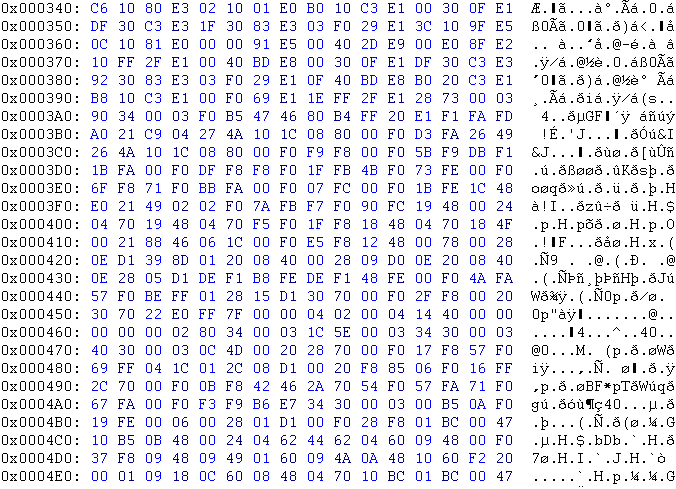
\includegraphics[width=12cm]{ch-bases/img/hex.png}\\
        \caption*{Un éditeur hexadécimal montre le contenu d'un fichier, d'un disque dur, ou de la RAM d'un ordinateur. La première colonne indique l'adresse,
            puis 16 octets écrits en hexadécimal et enfin les caractères correspondants.}
    \end{center}
\end{figure}
\section{Hexadécimal et binaire : un mariage heureux}
Le grand avantage qu'apporte l'hexadécimal s'illustre facilement :

\begin{methode}[ 6 : passer de la base 2 à la base 16]
    \begin{tabbing}
        $(101101000011101)_2$	\=	$=(0101\ 1010\ 0001\ 1101)_2$\\
        \>	$=\left(\underbrace{0101}_5\ \underbrace{1010}_A\ \underbrace{0001}_1\ \underbrace{1101}_D\right)_2$\\
        \>	$=(5A1D)_{16}$
    \end{tabbing}
\end{methode}

\begin{methode}[ 7 : passer de la base 16 à la base 2]
    $(F7B)_{16}=\left(\underbrace{1111}_F\ \underbrace{0111}_7\ \underbrace{1011}_B\right)_2$
\end{methode}
\begin{figure}
    \begin{center}
        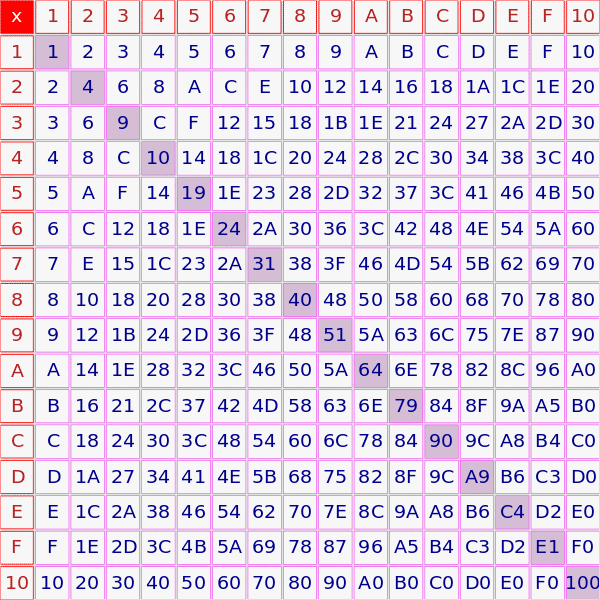
\includegraphics[width=10cm]{ch-bases/img/hexmult.png}\\
        \caption*{Table de multiplication hexadécimale.}
    \end{center}
\end{figure}


\section{Additions}

On pose l'opération à la main : c'est la même chose qu'en base 10.
\subsection*{En base 2}
La seule différence avec la base 10 c'est que deux 1 donnent $(2)_{10}$ donc $(10)_2$, donc un zéro et une retenue de 1.
Quand il y a deux 1 et une retenue de 1 en plus, cela donne $(3)_{10}$ donc $(11)_2$, donc un 1 et une retenue de 1.

\tabulardefault
\begin{exemple}[]
    \begin{center}
        \begin{tabular}{ccccccccc}
              &   &   & $_1$ & $_1$ & $_1$ &   &   &   \\
              & 1 & 1 & 0    & 1    & 0    & 1 & 0 & 1 \\
            + &   &   &      & 1    & 1    & 1 & 0 & 0 \\
            \hline
            = & 1 & 1 & 1    & 1    & 0    & 0 & 0 & 1 \\
        \end{tabular} \\[2em]
    \end{center}
\end{exemple}

\subsection*{En base 16}

C'est encore la même chose. Il faut bien se souvenir de la valeur de A, B, C, D, E et F.\\
Ajouter 8 et 3 ne provoque pas de retenue puisque $8+3=11$ et que $11$ est $B$ en base 16.\\
Dès que l'addition de 2 chiffres dépasse 15, il y aura une retenue : par exemple 9 et A donnent $(19)_{10}$, donc $(13)_{16}$. Ainsi on note 3 et une retenue de 1.

\begin{exemple}
    \begin{center}
        \begin{tabular}{ccccc}
              &   & $_1$ &   &   \\
              & 2 & 4    & 9 & 8 \\
            + & 1 & 7    & A & 3 \\
            \hline
            = & 3 & C    & 3 & B \\
        \end{tabular}
    \end{center}
\end{exemple}



\section{Exercices}

\begin{exercice}
    Donner l'écriture décimale des onze premières puissances de deux.
\end{exercice}

\begin{exercice}
    \begin{enumerate}
        \item 	Calculer $2^6+2^4+2^3+2^0$.
        \item 	En déduire l'écriture binaire de 89.
    \end{enumerate}
\end{exercice}

\begin{exercice}
    \begin{enumerate}
        \item 	Calculer $2^7+2^3+2^2+2^1$.
        \item 	En déduire l'écriture décimale de  $(1000 1110)_2$.
    \end{enumerate}
\end{exercice}

\begin{exercice}[]
    En utilisant la méthode 2, donner l'écriture binaire de
    \begin{enumerate}
        \item 	56
        \item 	35
        \item 	13
    \end{enumerate}
\end{exercice}

\begin{exercice}[]
    En utilisant la méthode 3, donner l'écriture binaire de
    \begin{enumerate}
        \item 	142
        \item 	273
        \item 	1000
    \end{enumerate}
\end{exercice}

\begin{exercice}
    \begin{itemize}
        \item 	Donner l'écriture décimale de $(1101\ 1010)_2$.
        \item 	Donner l'écriture binaire de 2016.
        \item 	Donner l'écriture hexadécimale de 2016.
    \end{itemize}
\end{exercice}

\begin{exercice}
    \begin{itemize}
        \item 	Donner les écritures décimales de $(11)_2$, $(111)_2$, $(1111)_2$.
        \item   Soit $n \in \N$, conjecturer la valeur de $ \left(\underbrace{1\ldots 1}_{n\textrm{ chiffres}}\right)_2$.
    \end{itemize}
\end{exercice}

\begin{exercice}
    Pour multiplier par dix un entier naturel exprimé en base dix, il suffit d'ajouter un 0 à sa
    droite, par exemple, $12\times 10 = 120$.\\
    Quelle est l'opération équivalente pour les entiers naturels exprimés en base deux?
\end{exercice}

\begin{exercice}
    \begin{enumerate}
        \item 	Donner l'écriture binaire de 174.
        \item 	Donner celle de 17.
        \item 	Poser l'addition de 174 et 17 en binaire.
        \item 	Donner l'écriture décimale du résultat et vérifier.
    \end{enumerate}
\end{exercice}

\begin{exercice}
    \begin{enumerate}
        \item 	Donner l'écriture hexadécimale de 1022.
        \item 	Donner celle de 3489.
        \item 	Poser l'addition de 1022 et 3489 en hexadécimal.
        \item 	Donner l'écriture décimale du résultat et vérifier.
    \end{enumerate}
\end{exercice}

\begin{exercice}[*]
    Le Roi d'un pays imaginaire fait frapper sa monnaie par 8 nains : chacun d'entre eux produit des pièces d'or de 10g chacune.\\

    Un jour, son Mage lui annonce : « Majesté, mon miroir magique m'a prévenu que certains de vos nains vous volent. Ils prélèvent 1g d'or sur chaque pièce qu'ils frappent. Pour vous aider à trouver les voleurs, voici une balance magique. Elle est précise au gramme près et peut peser autant que vous voulez. Malheureusement elle ne peut être utilisée qu'une fois.»\\

    Le lendemain, le Roi convoque les 8 nains en demandant à chacun d'apporter un coffre rempli de pièces d'or qu'il a frappées.\\
    On suppose que
    \begin{itemize}
        \item chaque nain dispose d'autant de pièces que nécessaire ;
        \item un nain honnête n'a que des pièces de 10g ;
        \item un nain voleur n'a que des pièces de 9g ;
    \end{itemize}

    Peux-tu aider le Roi pour démasquer les voleurs?
\end{exercice}